% % !TEX program = xelatex

% Author: Alexandr Korotkov
% https://github.com/ASKAlexAndr/bachelor-thesis

\documentclass[aspectratio=169]{beamer}
\hypersetup{pdfpagemode=FullScreen}
\title{Анализ алгоритмов глубокого машинного обучения  в задачах распознавания изображений}

\author[Коротков А.С.]{Александр Сергеевич Коротков}

\institute[]{Научный руководитель: Д.В. Матвеев}

\date{16.06.2020}

\usepackage{cmap}
\usepackage[english, russian]{babel}
\usepackage{csquotes}
\usepackage{filecontents}
\selectlanguage{english}
\usepackage[
    backend=biber,
    style=gost-numeric,
    maxcitenames=3,
    maxbibnames=4,
    minnames=3,
    movenames=false,
    ibidtracker=false,
    autolang=other,
    ]{biblatex}
\addbibresource{biblio/books.bib}
\usepackage{xunicode}
\usepackage{pdfpages}
\usepackage{xltxtra}

% Шрифты, xelatex
\defaultfontfeatures{Ligatures=TeX}
\setmainfont{Times New Roman} % Нормоконтроллеры хотят именно его
\newfontfamily\cyrillicfont{Times New Roman}
% \setsansfont{Liberation Sans} % Тут я его не использую, но если пригодится
\setmonofont{FreeMono} % Моноширинный шрифт для оформления кода

% % Формулы
\usepackage{mathtools,unicode-math} % Не совместим с amsmath
\setmathfont{XITS Math}             % Шрифт для формул: https://github.com/khaledhosny/xits-math
\numberwithin{equation}{section}    % Формула вида секция.номер

% Абзацы и списки
\usepackage{enumerate}   % Тонкая настройка списков
\usepackage{indentfirst} % Красная строка после заголовка
\usepackage{float}       % Расширенное управление плавающими объектами
\usepackage{multirow}    % Сложные таблицы

% Пути к каталогам с изображениями
\usepackage{graphicx} % Вставка картинок и дополнений
\graphicspath{{images/}}

% % Формат подрисуночных записей
\usepackage{chngcntr}

% % Сбрасываем счетчик таблиц и рисунков в каждой новой главе
% \counterwithin{figure}{section}
\counterwithin{table}{section}

% % Гиперссылки
\usepackage{hyperref}
\hypersetup{
    colorlinks, urlcolor={black}, % Все ссылки черного цвета, кликабельные
    linkcolor={black}, citecolor={black}, filecolor={black},
    pdfauthor={Александр Коротков},
    pdftitle={Анализ алгоритмов глубокого машинного обучения в задачах распознавания изображений}
}

% Оформление библиографии и подрисуночных записей через точку
\makeatletter
% \renewcommand*{\@biblabel}[1]{\hfill#1.}
\renewcommand*\l@section{\@dottedtocline{1}{1em}{1em}}
\def\redeflsection{\def\l@section{\@dottedtocline{1}{0em}{10em}}}
\makeatother

\renewcommand{\baselinestretch}{1.5} % Полуторный межстрочный интервал
\parindent 1.27cm % Абзацный отступ

\sloppy             % Избавляемся от переполнений
\hyphenpenalty=1000 % Частота переносов
\clubpenalty=10000  % Запрещаем разрыв страницы после первой строки абзаца
\widowpenalty=10000 % Запрещаем разрыв страницы после последней строки абзаца

% Отступы у страниц
\usepackage{geometry}
\geometry{left=3cm}
\geometry{right=2cm}
\geometry{top=2cm}
\geometry{bottom=2cm}

% Списки
\usepackage{enumitem}
\setlist[enumerate,itemize]{leftmargin=12.7mm} % Отступы в списках

\makeatletter
    \AddEnumerateCounter{\asbuk}{\@asbuk}{м)}
\makeatother
\setlist{nolistsep}                           % Нет отступов между пунктами списка
% \renewcommand{\labelitemi}{--}                % Маркер списка --
\renewcommand{\labelenumi}{\asbuk{enumi})}    % Список второго уровня
\renewcommand{\labelenumii}{\arabic{enumii})} % Список третьего уровня

% Содержание
\usepackage{tocloft}
\renewcommand{\cfttoctitlefont}{\hspace*{\fill}\bfseries}
\renewcommand{\cftaftertoctitle}{\hspace*{\fill}}
\setcounter{tocdepth}{3}                            % Глубина оглавления, до subsubsection


% Формат подрисуночных надписей
\RequirePackage{caption}
\DeclareCaptionLabelSeparator{deffis}{ -- } % Разделитель
\DeclareCaptionLabelFormat{rtable}{\hfill #1~#2}
\captionsetup[figure]{justification=centering, labelsep=deffis, labelfont=bf, format=plain} % Подпись рисунка по центру
\captionsetup[table]{justification=centerlast, labelsep=newline, textfont=bf, labelformat=rtable, format=plain, position=above, margin=0em} 
\addto\captionsrussian{\renewcommand{\figurename}{Рис.}} % Имя фигуры

\newcommand{\addimg}[4]{ % Добавление одного рисунка
    \begin{figure}
        \centering
        \includegraphics[width=#2\linewidth]{#1}
        \caption{#3} \label{#4}
    \end{figure}
}
\newcommand{\addimghere}[4]{ % Добавить рисунок непосредственно в это место
    \begin{figure}[H]
        \centering
        \includegraphics[width=#2\linewidth]{#1}
        \caption{#3} \label{#4}
    \end{figure}
}
\newcommand{\addtwoimghere}[6]{ % Вставка двух рисунков
\begin{figure}[H]   
    \centering    
    \subcaptionbox{#2}{\includegraphics[width=.49\textwidth]{#1}}   
    % \hfill
    \subcaptionbox{#4}{\includegraphics[width=.49\textwidth]{#3}}
    \caption{#5}
    \label{#6}
\end{figure}
}
\usepackage[labelformat=simple, labelsep=period]{subcaption}
\newcommand{\addthreeimghere}[8]{ % Вставка трех рисунков
    \begin{figure}[H]   
        \centering    
        \subcaptionbox{#2}{\includegraphics[width=.3\textwidth]{#1}}   
        % \hfill
        \subcaptionbox{#4}{\includegraphics[width=.3\textwidth]{#3}}
        % \hfill
        \subcaptionbox{#6}{\includegraphics[width=.3\textwidth]{#5}}
        \caption{#7}
        \label{#8}
    \end{figure}
}


% % Заголовки секций в оглавлении в верхнем регистре
% \usepackage{textcase}
% \makeatletter
% \let\oldcontentsline\contentsline
% \def\contentsline#1#2{
%     \expandafter\ifx\csname l@#1\endcsname\l@section
%         \expandafter\@firstoftwo
%     \else
%         \expandafter\@secondoftwo
%     \fi
%     {\oldcontentsline{#1}{#2}}
%     {\oldcontentsline{#1}{#2}}
% }
% \makeatother

% Оформление заголовков
\usepackage[compact, explicit]{titlesec}
\titleformat{\section}{}{}{12.5mm}{\bfseries\centering{\thesection\quad{#1}}\vspace{1.5em}}
\titleformat{\subsection}[block]{\bfseries\centering\vspace{1em}}{}{12.5mm}{\thesubsection\quad#1\vspace{1em}}
\titleformat{\subsubsection}[block]{\bfseries\centering\vspace{1em}\normalsize}{}{12.5mm}{\thesubsubsection\quad#1\vspace{1em}}
\titleformat{\paragraph}[block]{\normalsize\centering}{}{12.5mm}{#1}
% Секции без номеров (введение, заключение...), вместо section*{}
\newcommand{\anonsection}[1]{
    \phantomsection % Корректный переход по ссылкам в содержании
    \paragraph{\bfseries{{#1}}\vspace{1em}}
    \addcontentsline{toc}{section}{#1}
}

% Секция для аннотации (она не включается в содержание)
\newcommand{\annotation}[1]{
    \paragraph{\bfseries{{#1}}\vspace{1em}}
}

% Секции для приложений
\newcommand{\appsection}[1]{
    \phantomsection    
    \paragraph{\hfill\bfseries{{#1}}}
    \addcontentsline{toc}{section}{{#1}}
}

\usepackage{lastpage} % Подсчет количества страниц

% \setcounter{page}{2}  % Начало нумерации страниц

% \usepackage{lastbib} % Кол-во источников

\usepackage{totcount}
\usepackage[figure, table]{totalcount}

\newtotcounter{citnum} %% Счётчик библиографии
\AtEveryBibitem{\stepcounter{citnum}}

\regtotcounter{section}

\usepackage{listings} % Оформление исходного кода
\lstset{
    basicstyle=\small\ttfamily, % Размер и тип шрифта
    breaklines=true,            % Перенос строк
    tabsize=2,                  % Размер табуляции
    frame=single,               % Рамка
    literate={--}{{-{}-}}2,     % Корректно отображать двойной дефис
    literate={---}{{-{}-{}-}}3, % Корректно отображать тройной дефис
    language=Python,            % Язык программирования
    numbers=left,               % Нумерация строк
}

% Графики и таблицы
\usepackage{tikz}
\usepackage{pgfplots}
\usetikzlibrary{matrix, positioning}
\usepackage{bm}
\usepackage{relsize}

\usepackage{array, makecell}
\usepackage{xfrac}
\usepackage{multirow}

% Нейросети
\usepackage{neuralnetwork}

\newcommand{\x}[2]{$x_#2$}
\newcommand{\y}[2]{$\hat{y}_#2$}
\newcommand{\hfirst}[2]{\small $h_#2$}

\usepackage[ruled]{algorithm2e} % Подключаем преамбулу

\begin{document}
\maketitle
\begin{frame}{Цели и задачи работы}
    \textbf{Цель:} Изучить и проанализировать применение алгоритмов глубокого машинного обучения в задачах распознавания изображений \\
    \textbf{Задачи: }
    \begin{itemize}
        \item Изучить теоретический материал про обучение глубоких нейронных сетей и их применение в классификации изображений
        \item Изучить документацию библиотеки Tensorflow.
        \item Изучить вопрос диагностики COVID-19 по рентгеновским снимкам грудной клетки.
        \item Разработать и обучить различные модели сверточных нейронных сетей на наборе рентгеновских снимков.
        \item Сравнить точности работы реализованных нейронных сетей.
    \end{itemize}
\end{frame}

\begin{frame}{Сверточные нейронные сети}
    \begin{columns}[T]
        \begin{column}{.4\paperwidth}
            \centering
            \begin{figure}[H]
\centering
\begin{tikzpicture}

	\matrix (mtr) [matrix of nodes,row sep=-\pgflinewidth, nodes={draw}]
	{
		0 & 1 & 1 & |[fill=red!30]| 1 & |[fill=red!30]| 0 & |[fill=red!30]| 0 & 0\\
		0 & 0 & 1 & |[fill=red!30]| 1 & |[fill=red!30]| 1 & |[fill=red!30]| 0 & 0\\
		0 & 0 & 0 & |[fill=red!30]| 1 & |[fill=red!30]| 1 & |[fill=red!30]| 1 & 0\\
		0 & 0 & 0 & 1 & 1 & 0 & 0\\
		0 & 0 & 1 & 1 & 0 & 0 & 0\\
		0 & 1 & 1 & 0 & 0 & 0 & 0\\
		1 & 1 & 0 & 0 & 0 & 0 & 0\\
	};

	\draw[very thick, red] (mtr-1-4.north west) rectangle (mtr-3-6.south east);

	\node [below= of mtr-5-4.south] (lm) {$\bf I$};

	\node[right = 0.2em of mtr] (str) {$*$};

	\matrix (K) [right=0.2em of str,matrix of nodes,row sep=-\pgflinewidth, nodes={draw, fill=blue!30}]
	{
		1 & 0 & 1 \\
		0 & 1 & 0 \\
		1 & 0 & 1 \\
	};
	\node [below = of K-3-2.south] (lk) {$\bf K$};

	\node [right = 0.2em of K] (eq) {$=$};

	\matrix (ret) [right=0.2em of eq,matrix of nodes,row sep=-\pgflinewidth, nodes={draw}]
	{
		1 & 4 & 3 & |[fill=green!30]| 4 & 1\\
		1 & 2 & 4 & 3 & 3\\
		1 & 2 & 3 & 4 & 1\\
		1 & 3 & 3 & 1 & 1\\
		3 & 3 & 1 & 1 & 0\\
	};
	\node [below = of ret-4-3.south] (lim) {${\bf I} * {\bf K}$};

	\draw[very thick, green] (ret-1-4.north west) rectangle (ret-1-4.south east);

	\draw[densely dotted, blue, thick] (mtr-1-4.north west) -- (K-1-1.north west);
	\draw[densely dotted, blue, thick] (mtr-3-4.south west) -- (K-3-1.south west);
	\draw[densely dotted, blue, thick] (mtr-1-6.north east) -- (K-1-3.north east);
	\draw[densely dotted, blue, thick] (mtr-3-6.south east) -- (K-3-3.south east);

	\draw[densely dotted, green, thick] (ret-1-4.north west) -- (K-1-1.north west);
	\draw[densely dotted, green, thick] (ret-1-4.south west) -- (K-3-1.south west);
	\draw[densely dotted, green, thick] (ret-1-4.north east) -- (K-1-3.north east);
	\draw[densely dotted, green, thick] (ret-1-4.south east) -- (K-3-3.south east);

	\matrix (K) [right=0.2em of str,matrix of nodes,row sep=-\pgflinewidth, nodes={draw, fill=blue!10}]
	{
		1 & 0 & 1 \\
		0 & 1 & 0 \\
		1 & 0 & 1 \\
	};

	\draw[very thick, blue] (K-1-1.north west) rectangle (K-3-3.south east);

\end{tikzpicture}
\caption{Операция свертки} \label{convolution}
\end{figure}    
        \end{column}
        \begin{column}{.5\paperwidth}
            \begin{table}[H]
  \centering
  \begin{tabular}{|c|c|c|c|}
    \hline    
    Сеть          & Top-1   & Top-5     \\
    \hline
    VGG-16        & 71.3\%	& 90.1\%    \\
    \hline
    VGG-19        & 71.3\%	& 90.0\%    \\
    \hline
    Inception V3  & 77.9\%	& 93.7\%    \\
    \hline
    % ResNet-50    & 25 636 712	         & 74.9\%	& 92.1\%    \\
    % \hline
    % ResNet-101   & 44 707 176	         & 76.4\%	& 92.8\%    \\
    % \hline
    % ResNet-152   & 60 419 944		       & 76.6\%	& 93.1\%    \\
    % \hline
    ResNet-50 V2  & 76.0\%	& 93.0\%    \\
    \hline
    ResNet-101 V2 & 77.2\%	& 93.8\%    \\
    \hline
    ResNet-152 V2 & 78.0\%	& 94.2\%    \\
    \hline
    DenseNet-121  & 75.0\%	& 92.3\%    \\
    \hline
    DenseNet-169  & 76.2\%	& 93.2\%    \\
    \hline
    DenseNet-201  & 77.3\%	& 93.6\%    \\
    \hline
  \end{tabular}
\end{table}
        \end{column}
    \end{columns}   
\end{frame}

\begin{frame}{Задача диагностики COVID-19}
    \addthreeimghere{xray-normal}{Норма}{xray-pneumonia}{Пневмония}{xray-covid}{COVID-19}{Рентгеновские снимки грудных клеток}{xrays}
\end{frame}

\begin{frame}{Обучение сетей}
    \begin{columns}[T]
        \begin{column}{.4\paperwidth}
            \begin{figure}
                \centering
                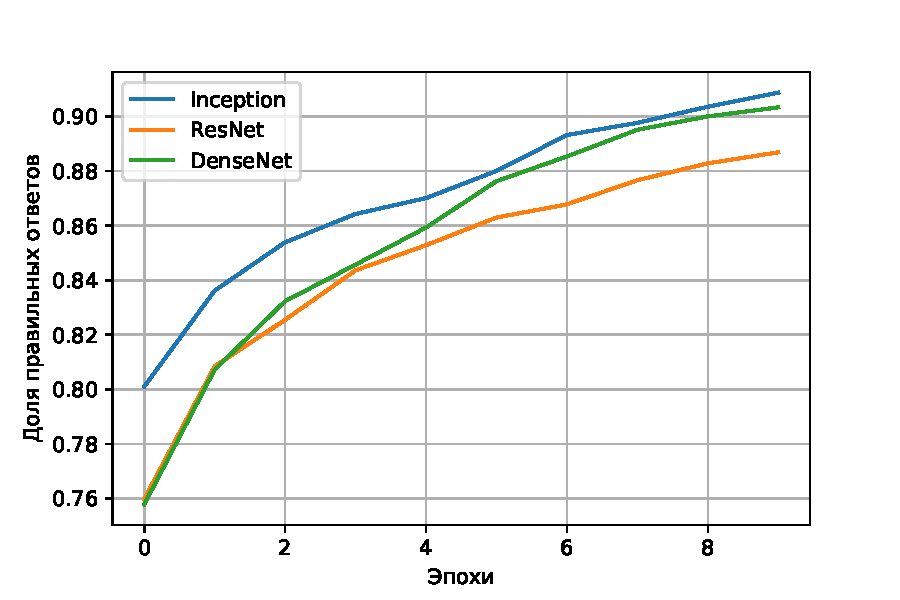
\includegraphics[width=\textwidth]{train_accuracy.pdf} 
                \caption{Обучение}
            \end{figure}            
        \end{column}
        \begin{column}{.4\paperwidth}
            \begin{figure}
                \centering                
                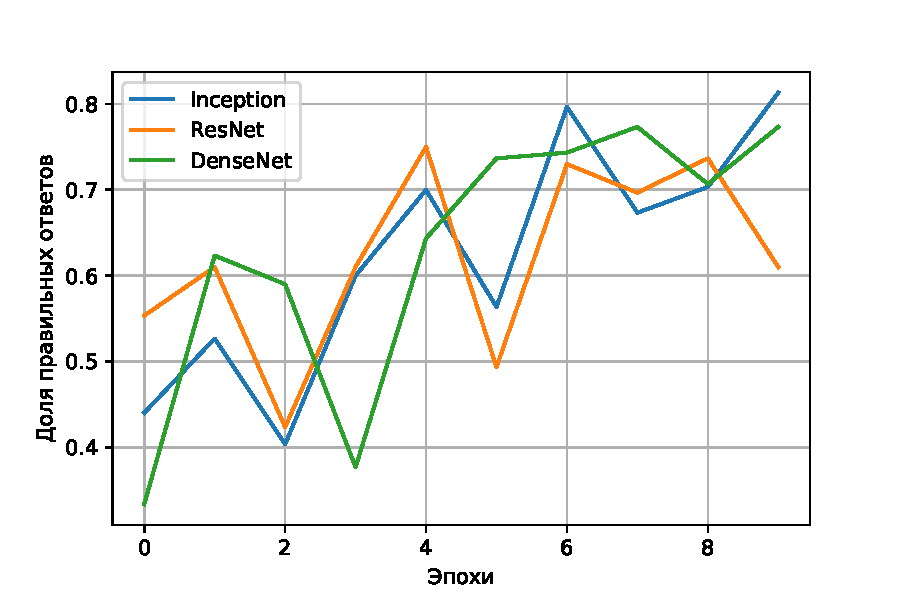
\includegraphics[width=\textwidth]{val_accuracy.pdf}
                \caption{Тестирование}
            \end{figure} 
        \end{column}
    \end{columns}   
\end{frame}
\begin{frame}{Заключение}
    Итоги:\\
    \begin{itemize}
        \item Глубокое обучение эффективно справляется с задачей классификации изображений. 
        \item Современные модели нейронных сетей обладают большим потенциалом для .
        \item Разработаны и обучены модели для диагностики COVID-19.
    \end{itemize}

    \vspace{2em}    
    Что дальше?
    \begin{itemize}
        \item Адаптировать модели для задачи.
        \item Увеличить базу данных и повысить длительность обучения.
        \item Проанализировать работу сетей по другим метрикам.
    \end{itemize}
\end{frame}
\begin{frame}
    \centering\Huge
    Спасибо за внимание!
\end{frame}
\end{document}